\chapter{PENGUJIAN DAN ANALISIS}
\label{chap:pengujiananalisis}

% Ubah bagian-bagian berikut dengan isi dari pengujian dan analisis
Pada penelitian ini dipaparkan hasil pengujian serta analisis yang dilakukan sesuai dengan desain sistem yang sudah dirancang pada bab sebelumnya. Dataset yang digunakan berasal dari \url{data.mendeley.com} ditambah dengan dataset yang berasal dari proses \textit{webcrawling} sendiri. Pengujian dilakukan dengan beberapa bagian sebagai berikut :

\begin{enumerate}[nolistsep]
    \item Pengujian Performa berdasar pada Penggalan Kata yang Diambil
    \item Pengujian Performa berdasarkan model BERT yang digunakan
    \item Pengujian Performa berdasarkan Pendekatan Cara \textit{Training}.
\end{enumerate}

Pada pengujian, masing - masing model menggunakan Google Collab dengan spesifikasi \textit{hardware} seperti yang dilampirkan pada tabel \ref{tab:specs_collab}

\begin{table}
    \caption{spesifikasi PC yang digunakan}
    \label{tab:specs_collab}
    \centering
    \begin{tabular}{|l|l|}
        \hline
        \textbf{Prosessor}            & 2 v-core Intel(R) Xeon(R) CPU @ 2.20GHz   \\ \hline
        \textbf{RAM}                  & Virtual Memory : 12GB                     \\ \hline
        \textit{\textbf{Storage}}     & SSD : 69GB                                \\ \hline
        \multirow{2}{*}{\textbf{GPU}} & Nvidia Tesla T4 16GB                      \\ \cline{2-2}
                                      & Nvidia K80 12GB                           \\ \hline
        \textbf{Sistem Operasi}       & Ubuntu 18.04.5 LTS (Bionic Beaver) 64-bit \\ \hline
    \end{tabular}
\end{table}

\section{Pengujian Performa berdasar pada Penggalan Kata yang Diambil}

Untuk saat ini, BERT hanya dapat memproses sebanyak 512 token sekaligus. Sehingga, untuk melakukan pemprosesan pada data dengan teks yang panjang, diperlukan pemotongan teks agar panjang teks menjadi sesuai.

Pengujian performa berdasar pada penggalan kata yang diambil ini bertujuan untuk mengetahui tingkat akurasi model BERT pada teks dengan cara pemotongan yang berbeda. Pembedaan ini dilakukan berdasarkan pada adanya berita yang menuliskan kesimpulan di awal, atau bisa juga menuliskan kesimpulan di akhir. Alternatif lain adalah mengambil sebagian teks di bagian awal dan mengambil sisanya di bagian akhir. Maka dari itu, dalam pengujian performa ini dilakukan dengan membagi teks pada beberapa cara memenggal kata, antara lain :

\begin{enumerate}[nolistsep]
    \item Mengambil bagian awal teks.
    \item Mengambil bagian akhir teks.
    \item Mengambil 129 token dari bagian awal teks dan 383 token dari bagian akhir teks.
\end{enumerate}

Dari total data yang berjumlah 1621 data, akan diambil 18\% nya sebagai dataset pengujian, sehingga berjumlah 292 dataset sebagai pengujian. Parameter pada pengujian untuk \textit{training} di atur agar sama untuk setiap pengujian, \textit{epoch} sebesar 7, \textit{leearning rate} sebesar 2e-5, dan \textit{epsilon} sebesar 1e-8, hal yang sama juga dilakukan pada model, pengujian ini menggunakan model BERT yang telah di-\textit{pre-trained} oleh Indobert. Untuk lebih jelasnya, silahkan lihat Tabel \ref{tab: truncate_param} yang berisi rincian parameter dan model yang digunakan untuk proses \textit{training}.

\begin{table}
    \caption{Konfigurasi Parameter Untuk Pengujian berdasarkan Pemotongan Kata}
    \label{tab: truncate_param}
    \centering
    \begin{tabular}{|l|l|}
        \hline
        \textit{\textbf{epoch}}          & 3                              \\ \hline
        \textit{\textbf{learning rates}} & 2e-5                           \\ \hline
        \textit{\textbf{epsilon}}        & 1e-4                           \\ \hline
        \textbf{model}                   & indobenchmark/indobert-base-p1 \\ \hline
    \end{tabular}
\end{table}

Keluaran dari model akan dibandingkan dengan label pada dataset, yang kemudian akan dihitung untuk menghasilkan \textit{confusion matrix}, \textit{recall, precision, accuracy} dan \textit{f1-score} sesuai dengan rumus yang telah dijelaskan pada bab tinjauan pustaka.

\subsection{Pengujian dengan Mengambil Bagian Awal Teks}

Terdapat beberapa ciri - ciri yang terdapat pada kebanyakan teks berita berbahasa Indonesia, salah satu dari ciri - ciri tersebut adalah menuliskan ringkasan berita pada paragraf awal kalimat. Format seperti ini biasanya cukup sering ditemui terutama pada berita yang memanfaatkan fitur halaman pada teks beritanya. Karenanya, pada jenis - jenis berita seperti ini, orang hanya perlu melihat beberapa kalimat awal untuk mengetahui apakah bahwa berita tersebut valid dan dapat dipercaya.

Seperti bisa dilihat pada tabel \ref{tab: const_awal}, dengan memotong teks berita pada bagian awal, didapatkan tingkat akurasi sebesar 89\% dengan nilai \textit{recall, precision, f1-score} kurang lebih sama. Selain itu, dapat dilihat juga pada kolom \textit{confusion matrix}, model yang sudah dibuat memiliki nilai FP dan FN yang sudah cukup sedikit. Namun, apabila melihat pada gambar \ref{fig: loss_const_awal}, terlihat bahwa model agak sedikit \textit{overfit}, sehingga terdapat kemungkinan akan memiliki tingkat akurasi yang lebih rendah pada saat implementasi.

\begin{table}
    \caption{Hasil Pengujian dengan Mengambil Awal Teks}
    \label{tab: const_awal}
    \centering
    \begin{tabular}{|l|l|l|}
        \hline
        \multicolumn{2}{|l|}{\textbf{Hasil Model}} & \textbf{Nilai}        \\ \hline
        \multirow{4}{*}{\textit{Confusion Matrix}} & TP             & 122  \\ \cline{2-3}
                                                   & FP             & 16   \\ \cline{2-3}
                                                   & TN             & 137  \\ \cline{2-3}
                                                   & FN             & 17   \\ \hline
        \multirow{2}{*}{\textit{Recall}}           & Hoax           & 89\% \\ \cline{2-3}
                                                   & Valid          & 88\% \\ \hline
        \multirow{2}{*}{\textit{Precision}}        & Hoax           & 90\% \\ \cline{2-3}
                                                   & Valid          & 88\% \\ \hline
        \multirow{2}{*}{\textit{F1-Score}}         & Hoax           & 89\% \\ \cline{2-3}
                                                   & Valid          & 88\% \\ \hline
        \multicolumn{2}{|l|}{\textit{Accuracy}}    & 89\%                  \\ \hline
    \end{tabular}
\end{table}

\begin{figure}[h]
    \begin{center}
        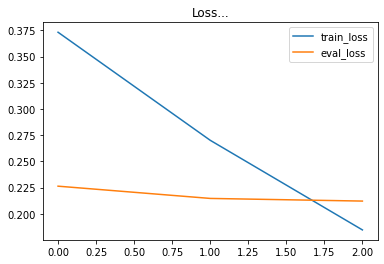
\includegraphics[width= 0.9\linewidth]{gambar/loss_concat_awal.png}
        \caption{Nilai \textit{Loss} saat Pengujian dengan Mengambil Bagian Awal Teks}
        \label{fig: loss_const_awal}
    \end{center}
\end{figure}


\subsection{Pengujian dengan Mengambil Bagian Akhir Teks}

Mirip seperti pengujian dengan mengambil bagian awal teks, terdapat ciri - ciri lain yang biasanya terdapat pada teks berita berbahasa Indonesia adalah adanya kesimpulan pada bagian akhir teks berita. Sehingga, setelah isi berita yang biasanya dibahas cukup dalam, pembaca dapat mengetahui bagaimana dan apa hubungan setiap informasi yang disajikan dengan peristiwa yang sedang dibahas dalam berita.

Dapat dilihat pada tabel \ref{tab: const_akhir}, model dengan cara memotong teks seperti ini berhasil mendapatkan tingkat akurasi sebesar 86\%. Namun, apabila melihat nilai \textit{recall} dan \textit{precision}-nya, ada indikasi bias dimana model lebih memiliki kecenderungan untuk mengeluarkan hasil hoaks bahkan pada berita valid sekalipun. Sedangkan, apabila melihat pada gambar \ref{fig: loss_const_akhir}, dapat dilihat bahwa baik nilai \textit{train loss} dan \textit{validation loss} sudah berada di titik optimal dan apabila dilakukan \textit{training} tambahan, akan membuat model \textit{overfit}.

\begin{table}
    \caption{Hasil Pengujian dengan Mengambil Akhir Teks}
    \label{tab: const_akhir}
    \centering
    \begin{tabular}{|l|l|l|}
        \hline
        \multicolumn{2}{|l|}{\textbf{Hasil Model}} & \textbf{Nilai}        \\ \hline
        \multirow{4}{*}{\textit{Confusion Matrix}} & TP             & 121  \\ \cline{2-3}
                                                   & FP             & 23   \\ \cline{2-3}
                                                   & TN             & 130  \\ \cline{2-3}
                                                   & FN             & 18   \\ \hline
        \multirow{2}{*}{\textit{Recall}}           & Hoax           & 88\% \\ \cline{2-3}
                                                   & Valid          & 84\% \\ \hline
        \multirow{2}{*}{\textit{Precision}}        & Hoax           & 85\% \\ \cline{2-3}
                                                   & Valid          & 87\% \\ \hline
        \multirow{2}{*}{\textit{F1-Score}}         & Hoax           & 86\% \\ \cline{2-3}
                                                   & Valid          & 86\% \\ \hline
        \multicolumn{2}{|l|}{\textit{Accuracy}}    & 86\%                  \\ \hline
    \end{tabular}
\end{table}

\begin{figure}[h]
    \begin{center}
        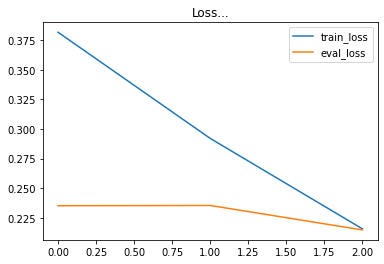
\includegraphics[width= 0.9\linewidth]{gambar/loss_concat_akhir.png}
        \caption{Nilai \textit{Loss} saat Pengujian dengan Mengambil Bagian Akhir Teks}
        \label{fig: loss_const_akhir}
    \end{center}
\end{figure}

\subsection{Pengujian dengan Mengambil Bagian Awal dan Akhir Teks}

Pengujian ini berdasarkan pada penelitian Chi Sun et al. yang menemukan bahwa dengan strategi pengambilan teks yang dibagi dua seperti ini akan dapat memberikan nilai akurasi yang lebih baik apabila dibandingkan dengan mengambil hanya di bagian awal maupun di bagian akhir saja \cite{sun2019fine}. Alasan dari penyebab lebih tingginya akurasi adalah karena dengan mengambil sebagian di awal maka sebagian dari ringkasan berita akan didapatkan, sedangkan mengambil sebagian di akhir adalah agar kesimpulan berita juga masuk ke dalam proses \textit{training}. Namun, pengujian tersebut dilakukan pada dataset teks berita berbahasa Inggris sehingga masih harus dilakukan pengujian lagi pada dataset teks berita berbahasa Indonesia.

\begin{table}[]
    \caption{Hasil Pengujian dengan Mengambil Tengah Teks}
    \label{tab: const_tengah}
    \centering
    \begin{tabular}{|l|l|l|}
        \hline
        \multicolumn{2}{|l|}{\textbf{Hasil Model}} & \textbf{Nilai}        \\ \hline
        \multirow{4}{*}{\textit{Confusion Matrix}} & TP             & 120  \\ \cline{2-3}
                                                   & FP             & 19   \\ \cline{2-3}
                                                   & TN             & 134  \\ \cline{2-3}
                                                   & FN             & 19   \\ \hline
        \multirow{2}{*}{\textit{Recall}}           & Hoax           & 88\% \\ \cline{2-3}
                                                   & Valid          & 86\% \\ \hline
        \multirow{2}{*}{\textit{Precision}}        & Hoax           & 88\% \\ \cline{2-3}
                                                   & Valid          & 86\% \\ \hline
        \multirow{2}{*}{\textit{F1-Score}}         & Hoax           & 88\% \\ \cline{2-3}
                                                   & Valid          & 86\% \\ \hline
        \multicolumn{2}{|l|}{\textit{Accuracy}}    & 87\%                  \\ \hline
    \end{tabular}
\end{table}

\begin{figure}[h]
    \begin{center}
        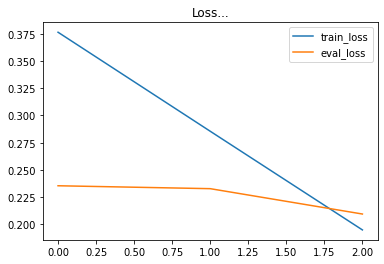
\includegraphics[width= 0.9\linewidth]{gambar/loss_concat_tengah.png}
        \caption{Nilai \textit{Loss} saat Pengujian dengan Mengambil Bagian Tengah Teks}
        \label{fig: loss_const_tengah}
    \end{center}
\end{figure}


\section{Pengujian Performa berdasarkan model BERT yang digunakan}

Terdapat banyak sekali model BERT yang sudah dibuat oleh berbagai orang di internet, ada model yang memiliki kemampuan \textit{multilanguage} sehingga bisa digunakan di berbagai bahasa sekaligus, namun kebanyakan model yang beredar adalah model yang menggunakan bahasa yang spesifik. Hal ini karena waktu \textit{pre-training} yang lebih singkat karena dataset yang lebih sedikit apabila dibandingkan model dengan kemampuan \textit{multilanguage} dan karena waktu \textit{pre-training} lebih sedikit, maka sumber daya yang digunakan juga menjadi lebih sedikit. Selain itu, dan hal ini adalah yang paling penting, hasil akurasi dari model yang hanya menggunakan 1 bahasa memiliki tingkat akurasi yang lebih tinggi apabila dibandingkan dengan model dengan banyak bahasa sekaligus.

Untuk model BERT yang menggunakan hanya bahasa Indonesia, terdapat 2 model yang bisa ditemukan pada waktu buku ini ditulis. Yang pertama dibuat oleh Bryan Wilie et al., sebagai bagian dari pengujian \textit{benchmark} berbahasa Indonesia dengan model BERT yang dilatih khusus dengan dataset berbahasa Indonesia juga \cite{wilie2020indonlu}. Hasil dari pengujian tersebut adalah model yang mereka buat berhasil memperoleh tingkat akurasi yang lebih tinggi apabila dibandingkan dengan model - model lain seperti XLM atau mBERT yang memiliki dukungan untuk melakukan tugas prediksi dengan banyak bahasa sekaligus \cite{wilie2020indonlu}. Model kedua dibuat oleh Candra Wirawan dengan melatih model pada 520MB data berasal dari Wikipedia Indonesia dan 1GB data berasal dari teks berita Indonesia. Sayangnya, tidak ada informasi lebih lanjut pada model ini selain data yang dipakai untuk \textit{pre-training}.

Selain model BERT yang hanya berisi bahasa Indonesia, kami juga melakukan percobaan pada model BERT yang mendukung \textit{multilanguage} dan model BERT yang hanya berisi bahasa Melayu. Bahasa Melayu dipilih karena kedekatan \textit{grammar} dan konteks dengan susunan kata berbahasa Indonesia. Untuk model yang mendukung \textit{multilanguage} kami menggunakan varian \textit{official} yang dibuat oleh Google, yaitu model \texttt{bert-multilingual-uncased} yang sudah mendukung 104 bahasa yang berasal dari Wikipedia. Sedangkan untuk model dengan bahasa Melayu, kami menggunakan model \texttt{bert-base-bahasa-standard-cased} yang sudah dilatih di beberapa sumber seperti Wikipedia, Wattpad, Berita, Sosial Media dan masih banyak lagi \cite{Malaya}

\begin{table}
    \centering
    \caption{Konfigurasi yang digunakan oleh model BERT yang digunakan}
    \label{tab:multi_bert_config}
    \begin{tabular}{|p{.5\linewidth}|c|l|p{.12\linewidth} |}
        \hline
        Model                          & epoch & dropout & learning rates \\ \hline
        bert-base-bahasa-standard-case & 4     & 0.2     & 2e-5           \\ \hline
        bert-base-multilingual-uncased & 4     & 0.2     & 2e-5           \\ \hline
        indobert-base-p1               & 3     & 0.1     & 2e-5           \\ \hline
        bert-base-indonesian-522M      & 3     & 0.1     & 2e-5           \\ \hline
        bert-base-indonesian-1.5G      & 3     & 0.2     & 2e-5           \\ \hline
    \end{tabular}
\end{table}

Untuk melakukan \textit{training}, sebelumnya kami mengatur konfigurasi yang akan digunakan oleh model BERT yang sudah disiapkan. Terdapat beberapa perbedaan pada konfigurasi seperti jumlah \textit{epoch} dan jumlah \textit{dropout}. Hal ini karena pada beberapa model, apabila menggunakan konfigurasi \textit{default} akan terjadi \textit{overfit} yang cukup parah.

\begin{figure}[h]
    \centering
    \subcaptionbox{\textit{Loss} pada model BERT Bahasa Melayu}{
        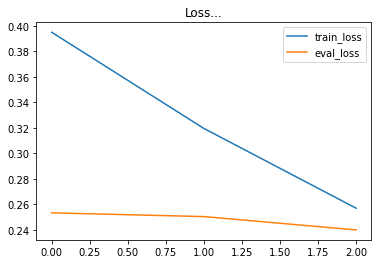
\includegraphics[width=.47\textwidth]{gambar/loss_bert_bahasa.png}
    }
    \subcaptionbox{\textit{Loss} pada model BERT \textit{Multilingual}}{
        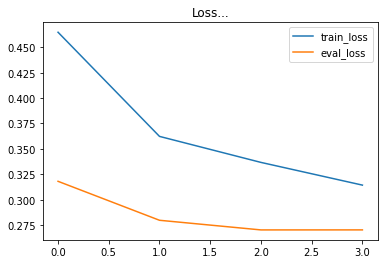
\includegraphics[width=.47\textwidth]{gambar/loss_bert_multilingual.png}
    }
    \subcaptionbox{\textit{Loss} pada model BERT IndoBERT}{
        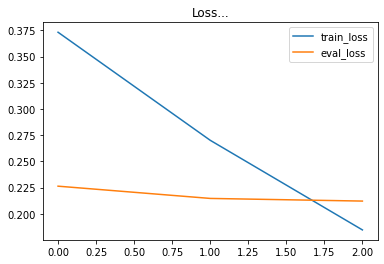
\includegraphics[width=.47\textwidth]{gambar/loss_concat_awal.png}
    }
    \subcaptionbox{\textit{Loss} pada model BERT Cahya 1.5GB}{
        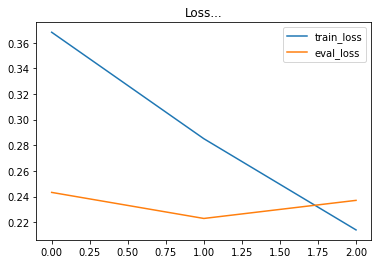
\includegraphics[width=.47\textwidth]{gambar/loss_cahya_bert_1,5.png}
    }
    \subcaptionbox{\textit{Loss} pada model BERT Cahya 522MB}{
        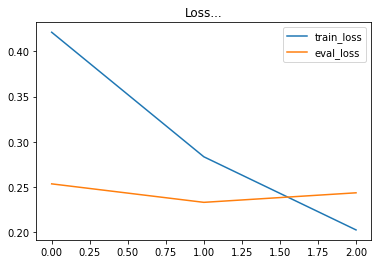
\includegraphics[width=.47\textwidth]{gambar/loss_cahya_bert_522.png}
    }
    \caption{\textit{Loss} pada Model BERT yang digunakan}
    \label{fig:loss_bert_model}
\end{figure}

Dapat dilihat pada gambar \ref{fig:loss_bert_model}, bahwa sebagian besar model BERT memiliki nilai \textit{loss} yang kurang lebih sama. Namun, apabila merujuk pada grafik \textit{loss} yang paling baik dimiliki oleh model \texttt{bert-base-bahasa-standard-case} yang merupakan model yang berisi bahasa Melayu, hal yang sama juga terjadi pada model \texttt{bert-base-multilingual-uncased} yang merupakan model dengan kemampuan \textit{multilanguage}. Sedangkan pada model - model lainnya, sudah mulai terlihat kenaikan pada \textit{validation loss} yang menunjukkan bahwa model sudah mulai mengalami \textit{overfit}.

\begin{figure}[h]
    \centering
    \subcaptionbox{\textit{Confusion Matrix} pada model BERT Bahasa Melayu}{
        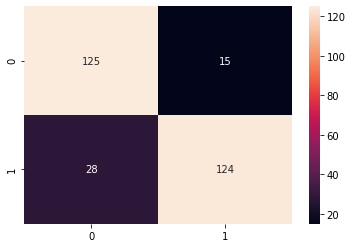
\includegraphics[width=.8\textwidth]{gambar/csf_mat_bert_bahasa.png}
    }
    \subcaptionbox{\textit{Confusion Matrix} pada model BERT \textit{Multilingual}}{
        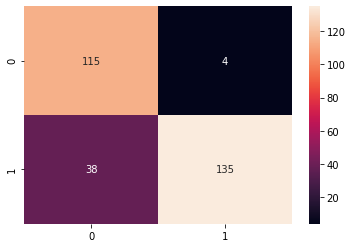
\includegraphics[width=.8\textwidth]{gambar/csf_mat_multilingual.png}
    }
    \caption{\textit{Confusion Matrix} pada Model BERT yang digunakan (bagian 1)}
    \label{fig:cfs_bert_model}
\end{figure}

\begin{figure}[h]
    \centering
    \subcaptionbox{\textit{Confusion Matrix} pada model BERT IndoBERT}{
        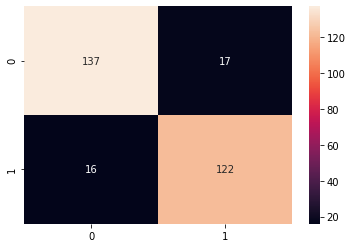
\includegraphics[width=.6\textwidth]{gambar/cfs_mat_concat_awal.png}
    }
    \subcaptionbox{\textit{Confusion Matrix} pada model BERT Cahya 1.5GB}{
        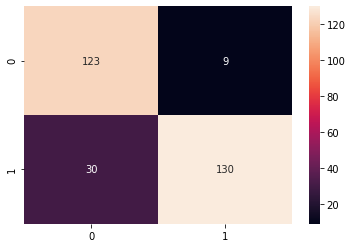
\includegraphics[width=.6\textwidth]{gambar/cfs_matrix_cahya_bert_1,5.png}
    }
    \caption{\textit{Confusion Matrix} pada Model BERT yang digunakan (bagian 2)}
    \label{fig:cfs_bert_model_2}
\end{figure}


\begin{figure}[h]
    \centering
    \subcaptionbox{\textit{Confusion Matrix} pada model BERT Cahya 522M}{
        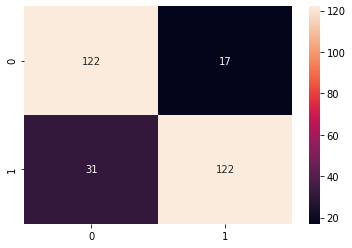
\includegraphics[width=.6\textwidth]{gambar/cfs_matrix_cahya_bert_522.png}
    }
    \caption{\textit{Confusion Matrix} pada Model BERT yang digunakan (bagian 3)}
    \label{fig:cfs_bert_model_3}
\end{figure}